\begin{figure}
  \center
  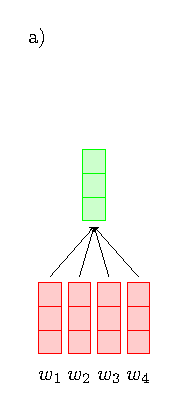
\includegraphics[scale=.7]{figures/avgsentencoder.pdf}
  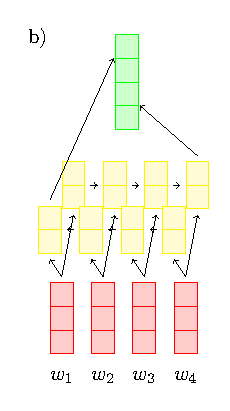
\includegraphics[scale=.7]{figures/rnnsentencoder.pdf}
  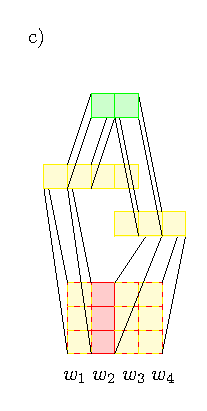
\includegraphics[scale=.7]{figures/cnnsentencoder.pdf}
  \caption{Sentence encoder architectures: a) averaging encoder, b) RNN encoder
           c) CNN encoder. Red indicates word embeddings, yellow indicates
           RNN hidden states or convolutional activations, and green 
           indicates the sentence embedding that is passed to the extractor
           module.}
    \label{fig:encoders}
\end{figure}

We treat each sentence $\sent = \{\wemb_1, \ldots, \wemb_{|\sent|}\}$ 
as a sequence of word embeddings, where $|\sent|$ is the total number of words
in the sentence. We experiment with three architectures for mapping sequences
of word embeddings to a fixed length vector: average pooling, RNNs, and CNNs.
See Figure~\ref{fig:encoders} for a diagram of the three encoders.

\textbf{Averaging Encoder} The averaging encoder (\textit{AVG}) is the simplest
method and has the added benfit of being parameter free. 
A sentence encoding is simply the average of its word embeddings: 
$\operatorname{enc}(\sent) = \frac{1}{|\sent|} \sum_{\wemb \in \sent} \wemb$.


\textbf{RNN Encoder} The \textit{RNN} sentence encoder uses the concatenation 
of the
final output states of a forward and backward RNN over the sentence's word
embeddings. We use a Gated Recurrent Unit (GRU) \cite{cho} for the RNN cell,
since it has fewer parameters than the equivalent LSTM but with similar 
performance. Formally, an \textit{RNN} sentence encoding is defined as
$\operatorname{enc}(s) = [\rSentVec_{|\sent|}; \lSentVec_1]$
where 
\begin{align} 
\rSentVec_i &= \rgru(w_i, \rSentVec_{i-1}) \\
\lSentVec_i &= \lgru(w_i, \lSentVec_{i+1}) 
\end{align}
for all $i \in 1, \ldots, |\sent|$. $\rgru$ amd $\lgru$ indicate the 
forward and backward GRUs respectively, and each have separate learned 
parameters.
The initial states $\rSentVec_0$ and $\lSentVec_{\sentSize + 1}$ are not 
learned and are set to zero vectors.

\textbf{CNN Encoder} The \textit{CNN} sentence encoder uses a series of 
convolutional feature maps to encode each sentence. This encoder is similar
to the convolutional architecture of \cite{kim} used for text classification
tasks and performs a series of ``one-dimensional'' convolutions over 
word embeddings. 
The \textit{CNN} encoder has hyperparameters
associated with the window sizes $\maxWindowSize \subset \mathcal{N}$ of the convolutional filter 
(i.e. the number of words associated with each convolution) and the number of 
feature maps $\maxFeatureMaps$ associated with each filter
(i.e. the output dimension of each 
convolution). 
The \textit{CNN} sentence encoding is computed as follows:
\begin{align}
 \specActivation_i &= \specConvBias 
    + \sum^\filterWindowSize_{j=1} \specConvWeight_j \cdot \wemb_{i + j -1}\\
  \specFeatureMap &= \max_{i\in 1,\dots, |\sent| - \filterWindowSize + 1} 
                      \relu\left(\specActivation_i\right) \\
 \senc(s) &= \left[\specFeatureMap | 
   \numFeatureMaps \in \{1, \ldots, \maxFeatureMaps\},
   \filterWindowSize \in \maxWindowSize
   \right]
\end{align}
where $\specConvBias\in\mathcal{R}$ and $\specConvWeight \in 
\mathcal{R}^{\filterWindowSize \times \wembdim}$ are learned bias and filter
weight parameters respectively, and $\relu(x) = \max(0, x)$ is the rectified
linear unit \cite{relu}.


